%% LyX 2.0.6 created this file.  For more info, see http://www.lyx.org/.
%% Do not edit unless you really know what you are doing.
\documentclass[11pt,english]{article}
\usepackage{helvet}
\renewcommand{\familydefault}{\sfdefault}
\usepackage[T1]{fontenc}
\usepackage[latin9]{inputenc}
\usepackage{geometry}
\geometry{verbose,tmargin=2cm,bmargin=2cm,lmargin=2cm,rmargin=2cm}
\usepackage{amsbsy}
\usepackage{graphicx}
\usepackage{babel}
\begin{document}

\section{Estimating the source field from the data}

Instead of using an explicit description of the railway source based
on some technical understanding of the railway installations, an alternative
attempt is to determine the source (or the sources) directly from
the data. A principal difficulty inherent to this approach is that
the observed fields depend on both the unknown source field and the
unknown conductivity structure. To deal with this problem, we shall
first make an assumption about the conductivity structure in order
to find a source field geometry that can account for the observations.
A second step would be to adjust the conductivity model to reduce
the residuals which can not be explained with our initial estimate
of the sources. These steps could be iterated until the data are explained.
There is of course no guarantee that this approach converges; however,
there is at least the hope, that this approach will help us to improve
our understanding of the railway source.

Similar problems exist in the field of global induction where the
objective is to determine mantle conductivity from magnetic fields
generated by inhomogeneous ionospheric or magnetospheric sources.
In theory, a solution to this problem can be obtained because internal
and external parts of the magnetic field can be separated from observations
with a dense array on an infinitely large or closed surface. Expansion
of the external part of the magnetic field into spherical harmonic
functions allows then to describe the source geometry as a function
of time, and the internal part arises due to induction phenomena within
the earth. With the knowledege of both the sources and the fields
of internal origin, the conductivity distribution can be determined
\cite{puethe2014}. In practice, the approach suffers from a sparse
distribution of observatories on the earth, which prohibits an exact
separation of the observed fields into parts of internal and external
origin. 

Here, we investigate two approaches to determine the source geometry.
The first approach is to find the sources by direct inversion of interstation
transfer functions. The second approach adopts multi-variate array
processing techniques, which have become popular in magnetotellurics
over the last years \cite{egbert1989}, but which have not yet been
applied to controlled or un-controlled source electromagnetic problems.
Array-processing techniques rely on the estimate of the principal
components of observations. We detail this approach below.


\subsection{Anna's inversion }


\subsection{Principal component analysis}

Our observations are the windowed and fourier-transformed recordings
of the horizontal electric field components at a number of recording
stations. The number of total channels corresponds to the number of
stations times two. Let us collect these responses $E_{n,i}$ for
all channels $n=1,\,...,\, N$ for a set of time windows $i=1,\,...,\, I$
in a $N\times I$ data matrix $\mathbf{X}$ as

\begin{equation}
\mathbf{X}=\left[\begin{array}{cccc}
E_{1,1} & E_{1,2} & \ldots & E_{1,I}\\
E_{2,1} & \ddots\\
\vdots &  & E_{n,i}\\
E_{N,1} &  &  & E_{N,I}
\end{array}\right]\,\,\,.\label{eq:PCA1}
\end{equation}
 Imagine that the observed fields in $\mathbf{X}$ result from linear
combinations of $P$ sources. It is clear, that the maximum number
of independent linear combinations of observations with our array
is $P$, corresponding to the number of independent sources. It can
then be shown, that all observed fields reside in a space that is
spanned by $P$ orthogonal coordinate axes. These coordinate axes
are the so-called principal components $\mathbf{U}$. In our case,
we can denote the principal components as principal electric fields,
and we aim at determining these from all observations in a statistically
robust way. Each particular observation (time window) results from
a particular linear combination and is reflected in the coeffcients
of a matrix $\mathbf{A}$. Therefore, it is useful to denote the elements
of $\mathbf{A}$ as polarization parameters. The principal component
analysis (PCA) yields exactly this decomposition of a data matrix:
\begin{equation}
\mathbf{X}=\mathbf{U}\mathbf{A}\label{eq:PCA2}
\end{equation}
The outcomes of a PCA of the data matrix $\mathbf{X}$ are thus the
number $P$ of independent observations, an orthogonal $P$-dimensional
coordinate system $\mathbf{U}$ in which all realizations must reside,
and the coordinates $\mathbf{A}$ of these observations in this coordinate
system. Other coordinate systems of the same dimension exist also;
for instance any rotation is allowed. Therefore the PCA is not unique. 

PCA is closely related to the singular value decomposition (SVD) of
a data matrix $\mathbf{X}$. Under ideal circumstances (noise-free
data and s small number of separable sources) the number of non-vanishing
singular values corresponds to the number of independent rows contained
in the $\mathbf{X}$. This is then the number of principal components.
The principal components $\mathbf{u}_{p}$ themselves are defined
as linear combinations of the data 
\begin{equation}
\mathbf{u}_{p}=\mathbf{X}\mathbf{a}_{p}^{T}\label{eq:PCA3}
\end{equation}
under the constraint that $\left\Vert \mathbf{a}_{p}\right\Vert =1$
and $\mathbf{u}{}_{p}^{T}\mathbf{u}{}_{q}=0$ for $p\neq q$. Here,
$\mathbf{u}_{p}$ and and $\mathbf{a}_{p}$ are $N\times1$ and $1\times I$
vectors, respectively. In turn, the data can written as linear combinations
of the principal components (cf. equation \ref{eq:PCA2}). The dimensions
of $\mathbf{U}=\left[\mathbf{u}_{1},\,...,\,\mathbf{u}_{P}\right]$
and $\mathbf{A}=\left[\mathbf{a}_{1}^{T},\,...,\,\mathbf{a}_{P}^{T}\right]^{T}$
are $N\times\left(P\leq N\right)$ and $P\times I$, respectively.
There is a maximum of $P=N$ principal components, but for low-dimensional
data, only the first $P\leq N$ components are required (this means
that there are less independent linear combinations than channels).
The decomposition of $\mathbf{X}$ is not unique, since $\mathbf{U}\mathbf{A}$
can be replaced with $\tilde{\mathbf{U}}\tilde{\mathbf{A}}$, where
$\tilde{\mathbf{U}}=\mathbf{U}\mathbf{B}^{-1}$ and $\tilde{\mathbf{A}}=\mathbf{A}\mathbf{B}$
and $\mathbf{B}$ is any non-singular $P\times P$ matrix. Therefore,
the SVD 
\begin{equation}
\mathbf{X}=\mathbf{U}\mathbf{S}\mathbf{V}^{T}\label{eq:PCA5}
\end{equation}
truncated at the $P-$th singular value yields only possible PCA representation.
For this set of principal components, $\mathbf{A}=\mathbf{S}\mathbf{V}^{T}$. 

It is important to understand that the principal components $\mathbf{u}_{p}$
can be thought of as independent representative observations of fields,
which contain as much information as all real observations (i.e. the
observations with field polarizations $\mathbf{a}_{i}$) taken together.
Therefore, to explain the entire set of observed data (i.e. all time
windows), it is sufficient to estimate the sources which generate
the fields $\mathbf{u}_{p}$. To illustrate this, we consider a simple
synthetic example in the sequel. 

For simplicity, we consider a non-inductive case. Then, for an electric
dipole at position $\mathbf{r}_{s}$ and with dipole moment $\mathbf{p}_{s}$,
the electric field at coordinate $\mathbf{r}$ is obtained from 
\begin{equation}
\mathbf{E}^{s}(\mathbf{r})=\frac{1}{4\pi\varepsilon_{0}}\left(3\frac{\mathbf{p}_{s}(\mathbf{r}-\mathbf{r}_{s})}{r^{5}}\cdot(\mathbf{r}-\mathbf{r}_{s})-\frac{1}{r^{3}}\mathbf{p}_{s}\right)\,\,\,,\label{eq:PCA6}
\end{equation}
where $r=\left|\mathbf{r}-\mathbf{r}_{s}\right|$. We denote the response
due to a unit dipole $\hat{\mathbf{p}}$ as $\hat{\mathbf{E}}(\mathbf{r})$,
where $\mathbf{E}^{s}(\mathbf{r})=p_{s}\hat{\mathbf{E}}^{s}(\mathbf{r})$
and $\mathbf{p}=p\hat{\mathbf{p}}$. Let us distribute a number of
$S_{0}$ electric dipoles and record the horizontal electric field
components with an array of $K$ stations. The total number of recording
channels is $N=2K$.

For the synthetic experiment, we transmit signal with random linear
combinations of all sources. Then, at a particular station at position
$\mathbf{r}$ the electric field is the superposition of contributions
from all source dipoles for a particular random realization $i$.
Hence, 
\begin{equation}
\mathbf{E}_{i}(\mathbf{r})=\sum_{s}r_{i,s}\mathbf{E}^{s}(\mathbf{r})=\sum_{s}r_{i,s}p_{s}\hat{\mathbf{E}}^{s}(\mathbf{r})\label{eq:PCA7}
\end{equation}
where the random number $r_{i,s}$ determines the strength of source
$s$. As before, we collect the responses $E_{n,i}$ at all channels
$n=1,\,...,\, N$ for all realizations $i=1,\,...,\, I$ to construct
a synthetic $N\times I$ data matrix $\mathbf{X}$ as 
\begin{eqnarray}
\mathbf{X} & = & \left[\begin{array}{cccc}
E_{1,1} & E_{1,2} & \ldots & E_{1,I}\\
E_{2,1} & \ddots\\
\vdots &  & E_{n,i}\\
E_{N,1} &  &  & E_{N,I}
\end{array}\right]+\boldsymbol{\delta}\nonumber \\
 & = & \left[\begin{array}{cccc}
\hat{E}_{1,1} & \hat{E}_{1,2} & \ldots & \hat{E}_{1,S}\\
\hat{E}_{2,1} & \ddots\\
\vdots &  & \hat{E}_{n,s}\\
\hat{E}_{N,1} &  &  & \hat{E}_{N,S}
\end{array}\right]\left[\begin{array}{cccc}
p_{1} &  &  & \mathbf{0}\\
 & \ddots\\
 &  & p_{s}\\
\mathbf{0} &  &  & p_{S}
\end{array}\right]\left[\begin{array}{cccc}
r_{1,1} & r_{1,2} & \ldots & r_{1,I}\\
r_{2,1} & \ddots\\
\vdots &  & r_{s,i}\\
r_{S,1} &  &  & r_{S,I}
\end{array}\right]+\boldsymbol{\delta}\nonumber \\
 & = & \hat{\mathbf{E}}\mathbf{p}\mathbf{R}+\boldsymbol{\delta}=\hat{\mathbf{E}}\mathbf{S}+\boldsymbol{\delta}\label{eq:PCA8}
\end{eqnarray}
where $\mathbf{S}=\mathbf{p}\mathbf{R}$ and $\boldsymbol{\delta}$
is a noise term. We denote $\mathbf{S}$ as the source parameters.

We apply a PCA on $\mathbf{X}$ and keep the $P$ dominant components,
i.e.
\begin{equation}
\mathbf{X}=\mathbf{U}\mathbf{A}=\hat{\mathbf{E}}\mathbf{S}+\boldsymbol{\delta}\,\,\,.\label{eq:PCA9}
\end{equation}
Here, we use the robust PCA code \texttt{robpca,} which is part of
the Matlab-based \texttt{LIBRA} library \cite{verboven2010}. Recall
that $\mathbf{A}$ contains the polarization parameters for each single
event. However, to represent the information contained in the observed
data, it sufficient to consider $P$ independent realizations. One
particular set of $P$ independent realizations, which would be generated
with the unknown source parameters $\mathbf{S}^{u}$ would correspond
to $\mathbf{A}=\mathbf{I}_{P\times P}$ being a unity matrix, i.e.
\begin{equation}
\mathbf{U}=\hat{\mathbf{E}}\mathbf{S}^{u}+\boldsymbol{\delta}\label{eq:PCA10}
\end{equation}
It means that this set of $P$ realizations would generate the fields
$\mathbf{u}_{p}$ at the actual receiver positions. We can now estimate
for each principal component $p=1,...,\, P$ the source parameters.
Let this problem be mixed-determined in the sense that we allow for
more unknown sources $S$ than independent components $P$. Then,
the damped least squares estimate for the source parameters is 
\begin{equation}
\mathbf{S}^{u,est}=(\hat{\mathbf{E}}^{T}\hat{\mathbf{E}}+\lambda\mathbf{I})^{-1}\hat{\mathbf{E}^{T}}\mathbf{U}\label{eq:SuestPCA11}
\end{equation}
where $\lambda$ is a regularization parameter. Each of the columns
of $\mathbf{S}^{u,est}$ then corresponds to the moments of each of
the $S$ sources, which, when superposed, give rise to the fields
given by the columns of $\mathbf{U}$. 

\begin{figure}
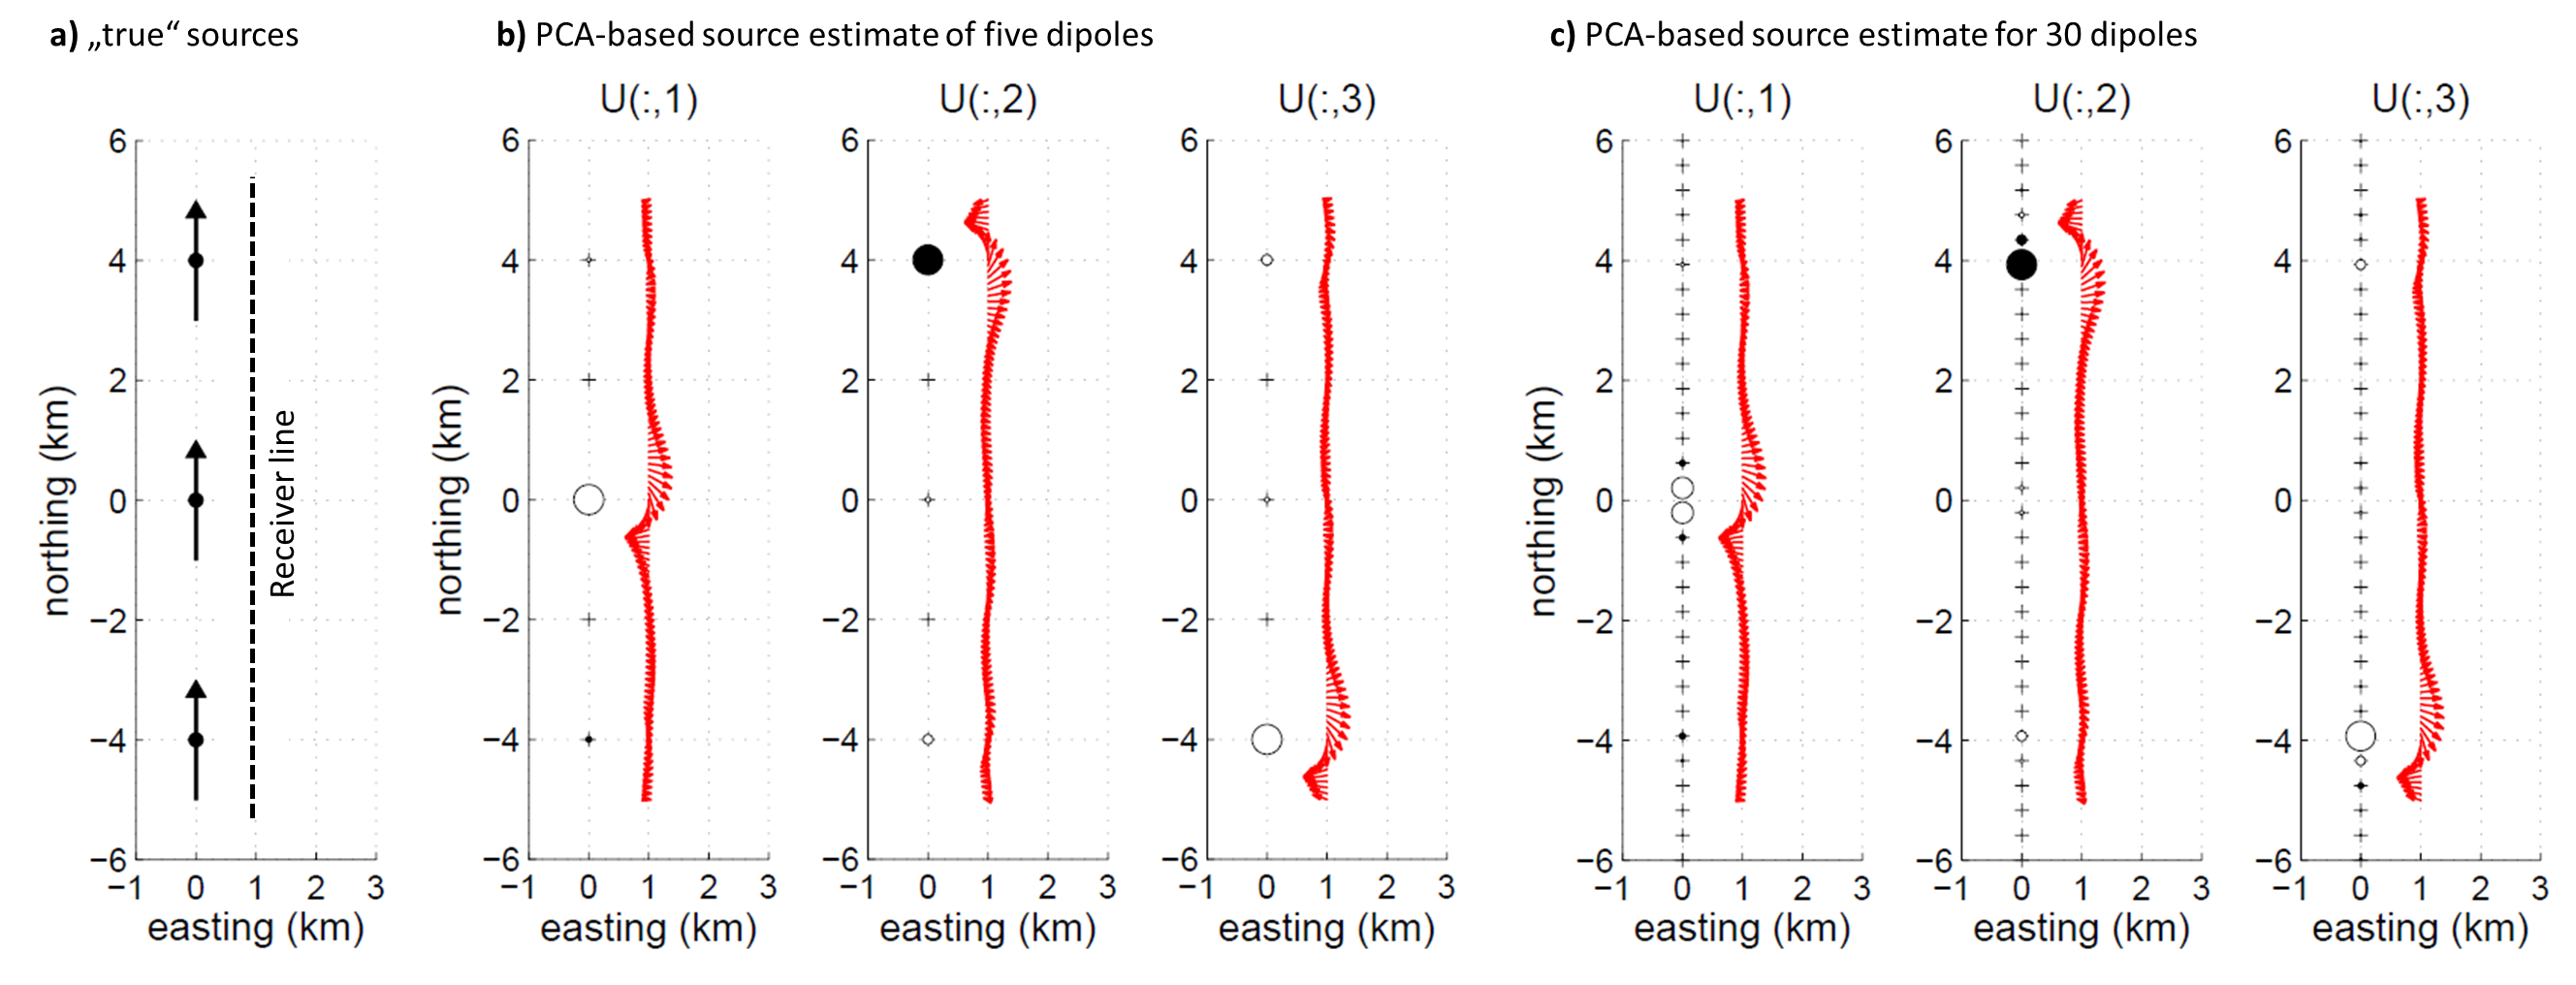
\includegraphics[width=1\textwidth]{PCA_syn2}

\caption{\label{fig:PCA1}PCA analysis applied to synthetic data. \textbf{a)}
Black arrows indicate position and orientation of three true source
dipoles. Thousand random linear combinations of the fields generated
by these sources have been collected along the receiver line (dashed
line). \textbf{b)} The PCA yields three independent source configurations,
which generate the principal electric fields plotted as red arrows
(corresponding to the columns of $\mathbf{U}$). The dipole moments
of five hypothetical sources (crosses corresspond to hypothetic source
positions) were estimated from the principal components. Source strength
estimates are depicted as circles with the diameter of each circle
corresponding to the estimated dipole strength; white and black colors
correspond to negative and positive dipole moments (i.e. the direction)
\textbf{c)} Same as in panel b), but with 30 hypothetic source locations.}
\end{figure}
Figure \ref{fig:PCA1} illustrates this approach. We use three point
dipoles and generate 1000 random realizations of fields to be observed
along a receiver line at $1\,\mbox{km}$ offset from the source line
(Figure \ref{fig:PCA1}a). With noise-free data, the PCA yields exactly
$P=3$ principal components. As outlined above, the principal components
can be conceived as independet representative fields for the data
set. Red arrows in Figure \ref{fig:PCA1}b,c depict these principal
fields. To solve for the source parameters, we place point dipoles
along the source line and compute the unit dipole responses for each
of the receivers. For the example in Figure \ref{fig:PCA1}b, we used
$S=5$ sources, three of which placed at the locations of the true
sources, and in the example in Figure \ref{fig:PCA1}c, we used $S=30$
sources. The source positions of these hypothetic sources are depicted
as crosses. The source strength estimates determined from expression
\ref{eq:SuestPCA11} correspond to the size of circles plotted on
top of the source line; white and black fillings correspond to negative
and positive moments, respectively. Note that in both examples, the
estimated sources which contribute to the principal components are
close to or exactly at the true source locations; however, each principle
component is shwon to be due a particular linear combination of the
true sources. This illustrates, that we can not identify each of the
true sources individually.

\begin{figure}
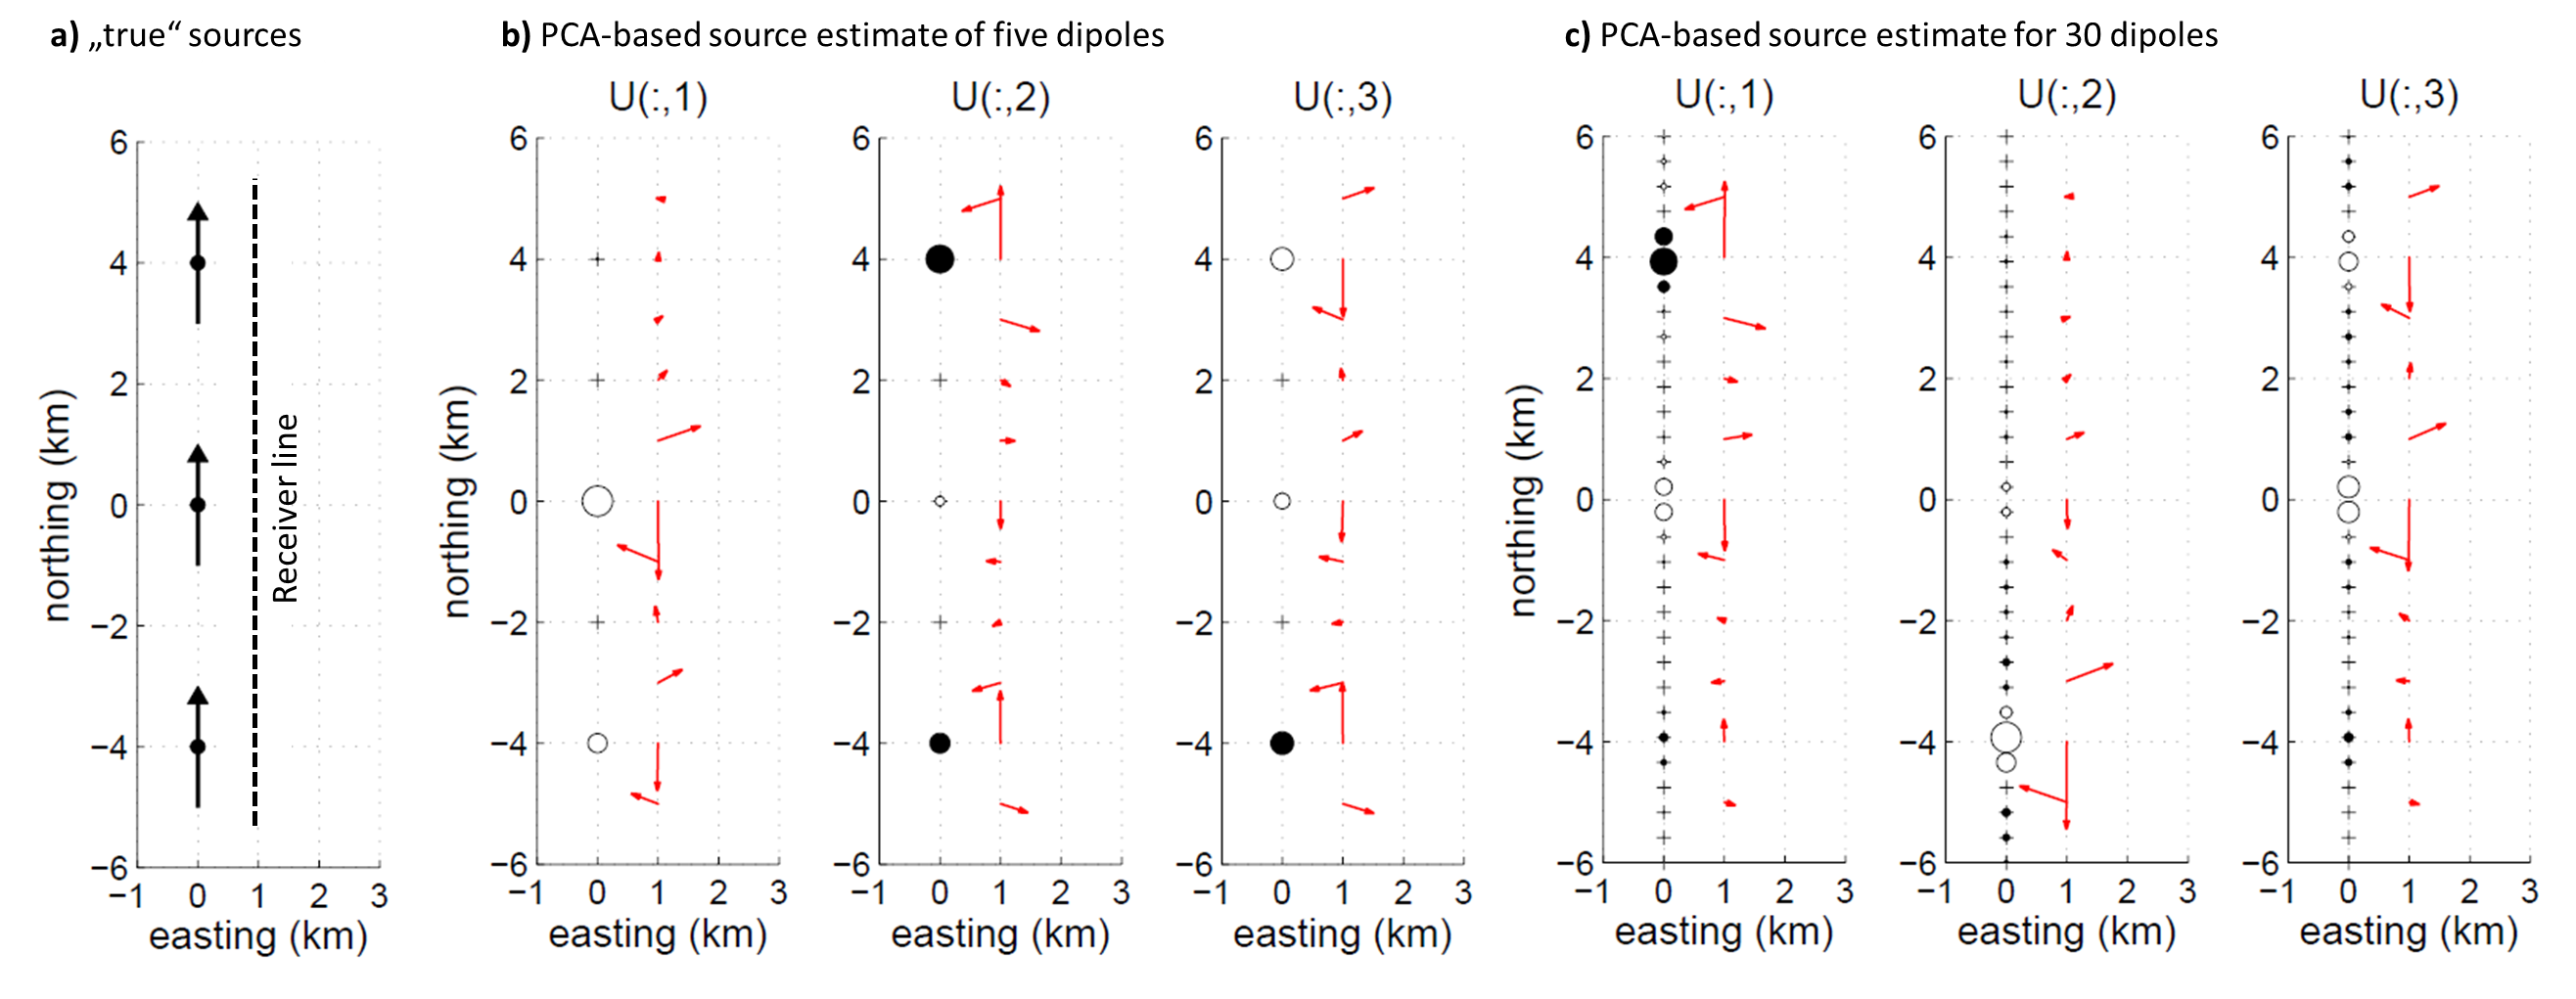
\includegraphics[width=1\textwidth]{PCA_syn3}

\caption{\label{fig:PCA2}Same as in Figure \ref{fig:PCA1}, but only 11 receivers
have been used for the PCA.}
\end{figure}
We have repeated the same experiment with a sparse subset of eleven
stations. The results are depcited in Figure \ref{fig:PCA2}. Even
though the principles fields lokk at a first glance spatially inconsistent,
the reconstruction of sources resembles the true sources. 

These synthetic examples suggest that the PCA analysis may be a useful
tool to extract information about the railway source from the observed
electric field data. We have started to apply this approach to the
real data, and we propose to pursue this approach further in this
project. 

\bibliographystyle{plain}
\bibliography{bibtex}

\end{document}
